\documentclass[11pt, a4paper]{article}

\usepackage[utf8]{inputenc}
\usepackage{geometry}
\geometry{margin=1in}
\usepackage{graphicx}
\usepackage{booktabs}
\usepackage{hyperref}
\usepackage{float}
\usepackage{caption}
\usepackage{fancyhdr}
\usepackage{titlesec}
\usepackage{enumitem}

\graphicspath{{../}}

\title{Bayesian Optimization Report \\ \Large Formula B -- Phase 1}
\author{}
\date{\today}

\begin{document}

\maketitle
\tableofcontents
\listoffigures
\listoftables
\newpage

\section{Introduction}
This report outlines the application of Bayesian Optimization to fine-tune the hyperparameter of \textbf{Formula B (Phase 1)}. This formula utilizes Harmonic Sequence Growth, scaling the array capacity inversely proportional to the resize count $k$. By automating the search through the parameter space using Gaussian Processes, we aim to uncover the mathematically optimal value for the harmonic coefficient $c$ ($c_0$) that perfectly balances memory waste, reallocation cost, and execution speed.

\section{Optimization Setup}

\subsection{Objective Function (J-Score)}
The optimizer minimizes a composite score ($J$), which normalizes the strategy's performance against standard baselines (Fixed 2.0x and Python list). The weighting is:
\begin{itemize}
    \item 40\% Memory Waste
    \item 40\% Total Elements Copied
    \item 20\% Execution Time
\end{itemize}

\subsection{Parameter Space \& Workload}
\begin{itemize}
    \item \textbf{Harmonic Coefficient ($c$)}: Explored continuous space between 0.1 and 10.0.
    \item \textbf{Evaluations}: 35 total iterations (10 initial random probes).
    \item \textbf{Workload}: 10,000,000 Uniform insertions.
\end{itemize}

\section{Optimization Results}

After 35 iterations, the Bayesian Optimization model successfully identified the optimal parameter for a 10M insertion workload. Because the search space is only 1-dimensional, the Gaussian Process was able to map the domain exhaustively.

\begin{table}[H]
\centering
\caption{Top 5 Configurations Discovered via Bayesian Optimization (Formula B)}
\label{tab:top_bo}
\begin{tabular}{cccccc}
\toprule
\textbf{Rank} & \textbf{$c$ Value} & \textbf{J-Score} & \textbf{Waste (\%)} & \textbf{Copied (M)} & \textbf{Time (ms)} \\
\midrule
% DATA_PLACEHOLDER_START
1 & 7.5873 & 0.5898 & 2.44 & 38.19 & $\sim 1460$ \\
2 & 7.3828 & 0.6144 & 2.57 & 40.40 & $\sim 1481$ \\
3 & 7.8189 & 0.6437 & 3.11 & 36.28 & $\sim 1495$ \\
4 & 5.6395 & 0.6445 & 1.33 & 73.27 & $\sim 1335$ \\
5 & 0.1029 & 0.6712 & 0.17 & 100.17 & $\sim 1319$ \\
% DATA_PLACEHOLDER_END
\bottomrule
\end{tabular}
\end{table}

\section{Graph Analysis}

To visualize the optimizer's path, we generated performance plots using the full 35-record history.

\subsection{Convergence Plot}
\begin{figure}[H]
    \centering
    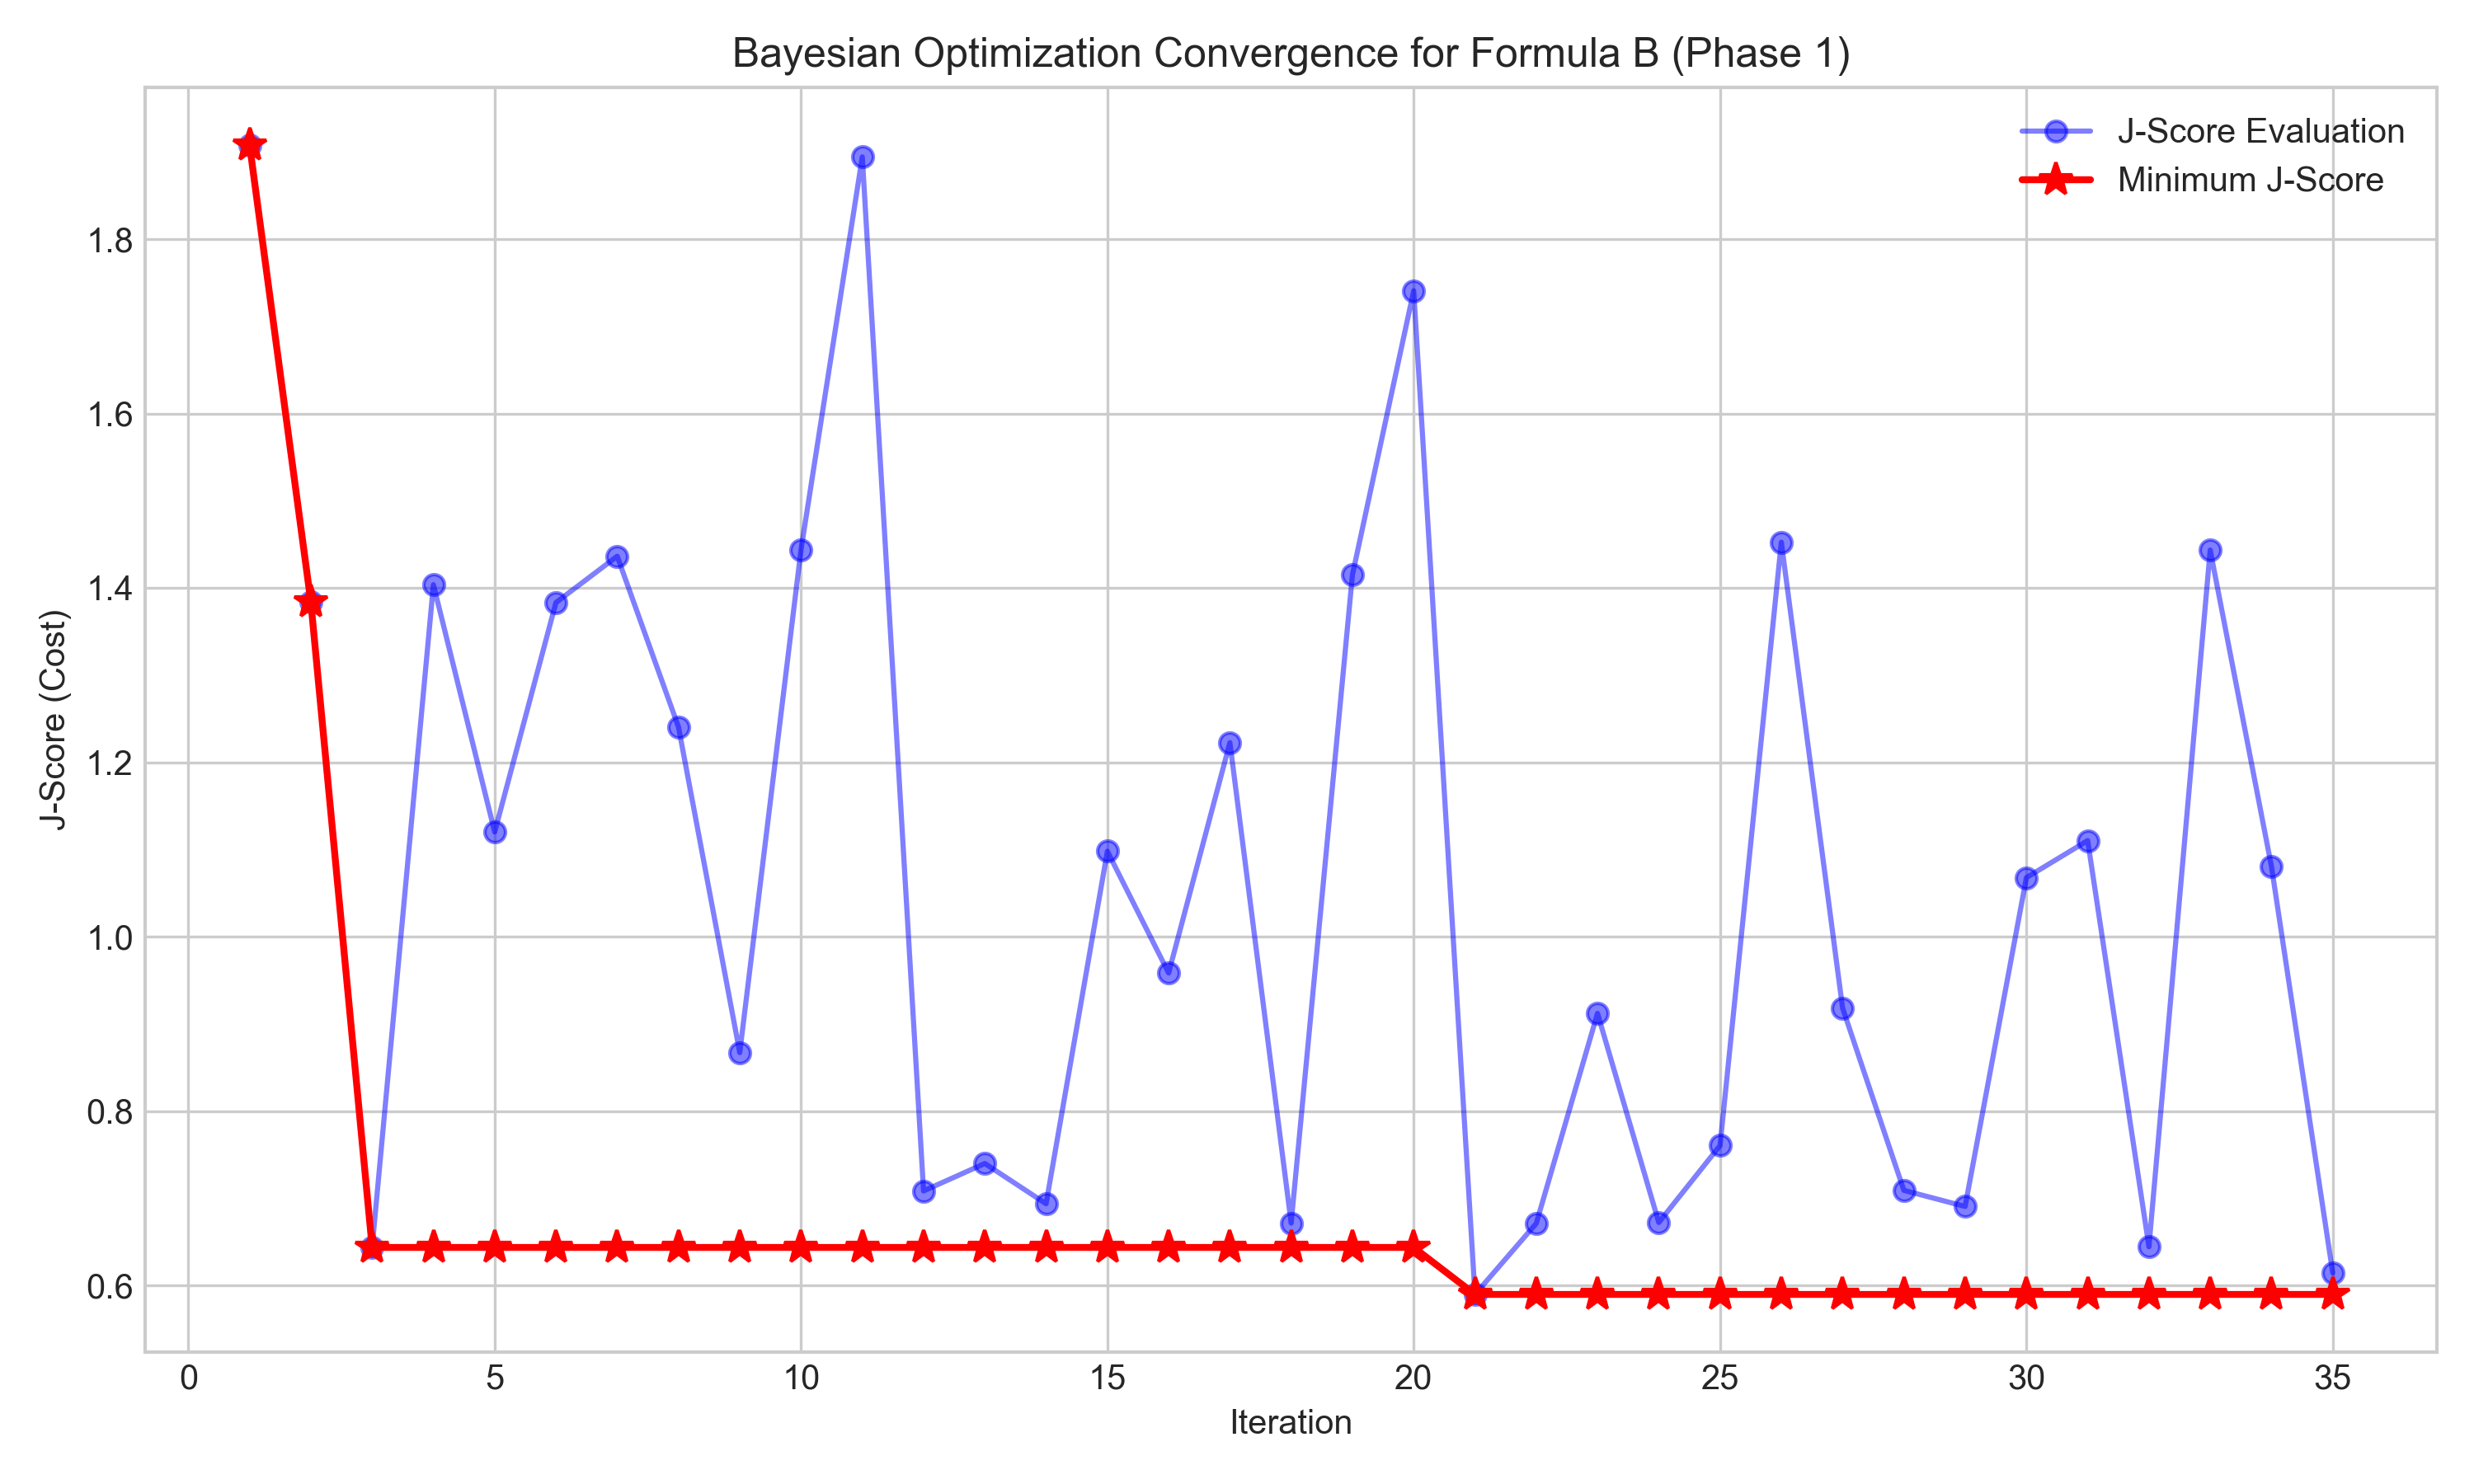
\includegraphics[width=0.9\textwidth]{bo_convergence.png}
    \caption{J-Score Convergence over 35 Iterations}
    \label{fig:convergence}
\end{figure}
Figure \ref{fig:convergence} illustrates the optimizer's progress. The blue line represents the $J$-Score evaluated at each iteration, while the red line tracks the minimum $J$-Score found so far.

\subsection{Parameter Space Exploration (1D Mapping)}
\begin{figure}[H]
    \centering
    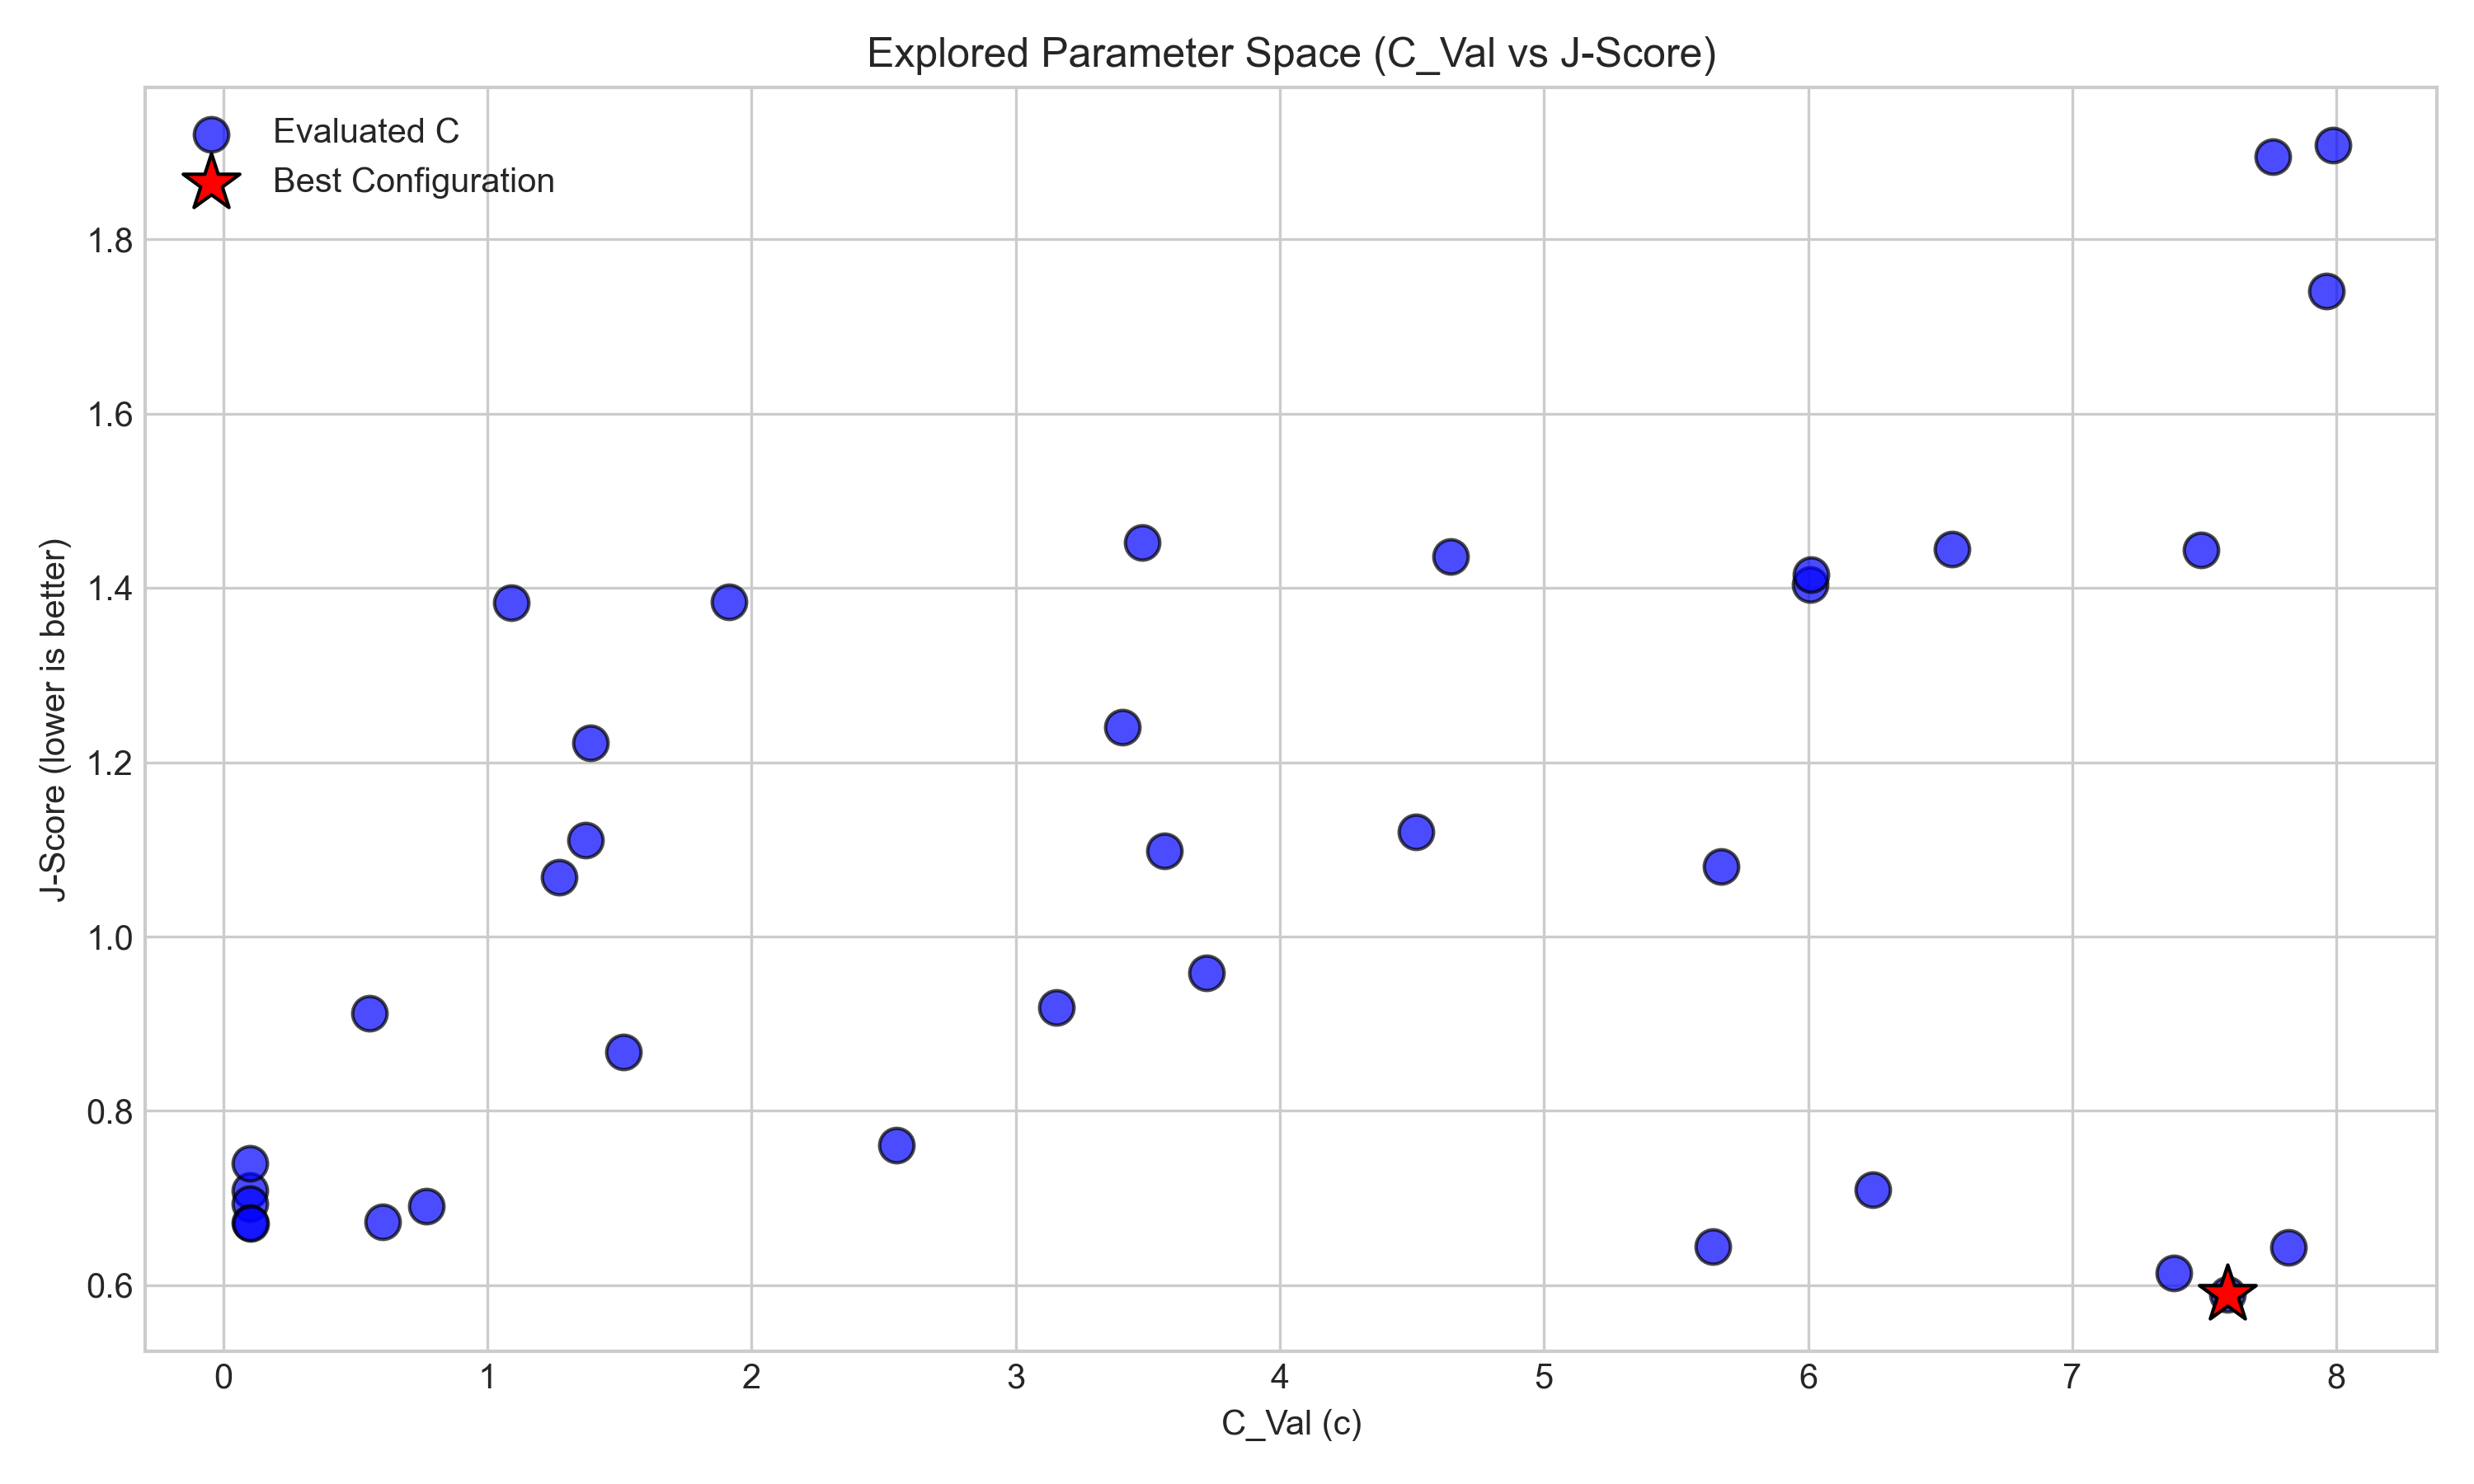
\includegraphics[width=0.9\textwidth]{bo_parameter_scatter.png}
    \caption{Explored Parameter Space ($c$ vs J-Score)}
    \label{fig:scatter}
\end{figure}
Figure \ref{fig:scatter} graphs the explored parameter $c$ against its resulting $J$-Score. Since this is a 1-dimensional search, this plot clearly reveals the landscape of the objective function and the global minimum (highlighted by the red star).

\end{document}
